\documentclass[10pt,twoside,slovak,a4paper]{article}
\usepackage[slovak]{babel}
\usepackage[utf8]{inputenc}
\usepackage{indentfirst}
\usepackage{graphicx}
\usepackage{hyperref}
\usepackage{amsmath}
\usepackage{cite}
\usepackage{url}

\graphicspath{{data}}
\pagestyle{headings}

\title{Paralelný web crawler\thanks{Semestrálny projekt v predmete Metódy inžinierskej práce ak. rok 2023/24, vedenie: Ing. Richard Marko, PhD.}}

\author{Peter Kapusta \\
	\small Slovenská technická univerzita v Bratislave \\
	\small Fakulta informatiky a informačných technológií \\
	\small \texttt{xkapustap@stuba.sk}
}

\begin{document}

\maketitle

\begin{abstract}
V článku je vysvetlené využitie paralelných web crawlerov, problematika komunikácie medzi jednotlivými procesmi a sú uvedené riešenia, ktoré sa momentálne využívajú.
\end{abstract}

\section{Úvod}

Vo všeobecnosti, web crawler je program, ktorý systematicky skenuje web, sťahuje webstránky a následne z nich extrahuje informácie, ktoré môže neskôr využiť napr. prehliadač. Cieľom je teda čo najefektívnejšie a najrýchlejšie objaviť čo najväčšie množstvo informácií. Hlavnou ťažkosťou je prehľadávanie HTML kódu a získavanie využiteľných odkazov, ktoré vedú k novým webstránkam. Čo ale robí paralelizované web crawlery špeciálnymi, je ich schopnosť súčasne získavať tieto dokazy z rôznych zdrojov, bez toho, aby sa osobitné procesy prekrývali – tým sa čo najoptimálnejšie využije maximálna rýchlosť sťahovania na danej siete. Internet môžeme vnímať ako orientovaný graf, ktorého vrcholy sú reprezentované jednotlivými webstránkami a hrany tvoria odkazy medzi nimi \cite{7148493}. Úlohou paralelného crawleru je teda prechádzať týmto grafom viacerými procesmi.

\newpage

\begin{figure}
	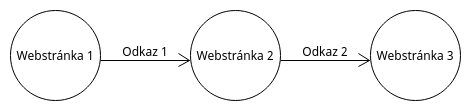
\includegraphics[width=\textwidth]{diagram1.png}
	\caption{Orientovaný graf reprezentujúci vzťah medzi webstránkami}
\end{figure}

\begin{figure}
	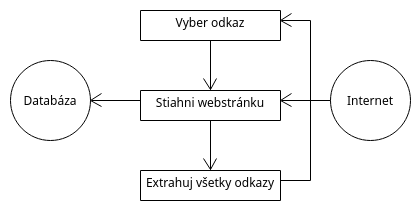
\includegraphics[width=\textwidth]{diagram2.png}
	\caption{Princíp získavania informácií web crawlerom \cite{sharma2011novel}}
\end{figure}

Matica:
$A=\begin{bmatrix}
1  & 2  & 3  & 4  \\
5  & 6  & 7  & 8  \\
9  & 10 & 11 & 12 \\
13 & 14 & 15 & 16 \\
17 & 18 & 19 & 20
\end{bmatrix}$

\vspace{\baselineskip}

Postupnosť:
\begin{equation*}
\left\{\frac{1}{n}\right\}^{\infty}_{n=1}=\left\{\frac{1}{1},\frac{1}{2},\frac{1}{3},\frac{1}{4},\frac{1}{5},\frac{1}{6},\frac{1}{7},\frac{1}{8},\frac{1}{9},\frac{1}{10},\frac{1}{11},\frac{1}{12},\frac{1}{13},\frac{1}{14},\frac{1}{15},\frac{1}{16},\frac{1}{17}\ldots\right\}
\end{equation*}

\section{Porovnanie rýchlosti}
Exituje mnoho spôsobov ako implementovať samotné procesy jednolivých web crawlerov. V tomto odseku, ale porovnáme rozdiely vo výkone web crawlerov, ktoré boli vytvorené pomocou procesov, threadov (vlákien) a systémového volania \texttt{epoll} (poskytovaného Linuxovým jadrom), napísané v programovacom jazyku C++ \cite{9648837}. \\

Jazyk C++ bol vybraný pre knižnicu \texttt{pthreads}, ktorá je v ňom dostupná \cite{9648837}. 

\section{Zloženie}

Paralelné web crawlery sa skladajú z viacerý komponentov, ktoré sa dajú zrealizovať viacerými spôsobmi. \cite{9645918} \cite{kausar2013web} % Vysvetliť, že jednotlivé crawlery môžu byť spustené na rôznych počítačoch \cite{sharma2011novel}

\begin{enumerate}
	\item Viacvláknový server - Koordinuje činnosť jednotlivých klientov.
	\item Klienty - Jednotlivé počítače, ktoré sťahujú webstránky.
	\item Crawlovací systém - Program, ktorý zaisťuje aby webstránky neboli sťahované opakovane.
\end{enumerate}

\section{Existujúce riešenia}
	\subsection{Crawler typu „C-procs" \cite{sharma2011novel}} % Vysvetliť fungovanie a výhody podľa zdroja

\newpage

\nocite{*}
\bibliography{literatura}
\bibliographystyle{unsrt}

\end{document}
